\section{Methodology}

\subsection{Description of the data}
% Data verzameling en beschrijving van de data
% Hoe is de data verzameld, en hoe heb jij die data verkregen?
% Wat staat er in de data? Niet alleen maar een technisch verhaal, maar ook inhoudelijk. DE lezer moet een goed idee krijgen over de technische inhoud en wat het betekent.
For classifying fake news, Wang's Liar dataset will be used \cite{wang2018}. 
The Liar dataset contains 12.791 short statements from Politifact.com, which are labeled manually by a Politifact.com editor on truthfulness. 
The statements are an average of 18 tokens long, and the topics vary from different political subjects, as can be seen in figure 1\todo{Check whether this number is still correct}.
Truthfulness is evaluated by assigning one of 6 labels, ranging from \textit{pants-on-fire} to \textit{true}. 
The distribution of statements across the original 6 labels can be seen in table 2\todo{Check whether this number is still correct}.

\begin{figure}[h]
    \centering
    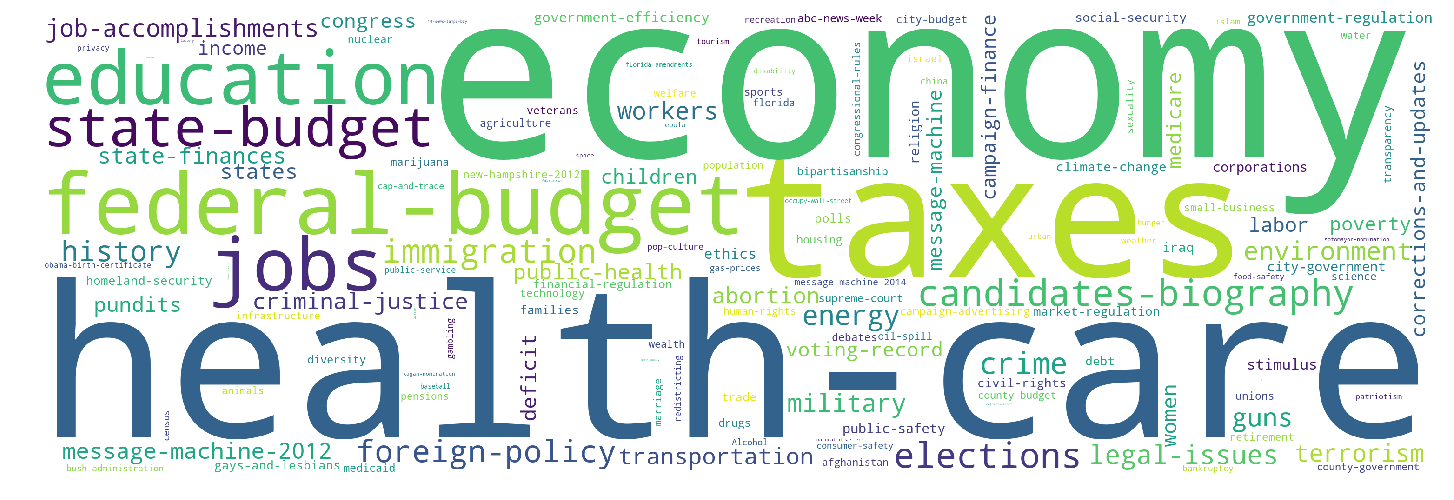
\includegraphics[scale=0.25]{subjectwordcloud}
    \caption{An overview of all statement topics in the Liar dataset.}
\end{figure}

For each statement, the dataset contains an id, a label, a subject, a speaker, the function title of the speaker, the affiliated state and political affiliation, the context of the statement and a vector with a truthfulness history.
An example of such a data entry can be seen in table 1.\todo{Check whether this number is still correct}
Wang introduced this truthfulness history to boost the prediction scores, as speakers with a track record of lying are expected to have a lower chance of speaking the truth when classifying new statements.
However, for our application we are only interested in the statement itself and its corresponding label. 
Due to cheapness and spreadability, a large amount of fake news is spread over social media \cite{shu2017}. 
This means author information and metadata will not readily be available in real world circumstances.

\begin{table}[]
    \centering
    \begin{tabular}{ll}
        \hline
        id                     & 11044.json                                                      \\ \hline
        label                  & pants-fire                                                      \\ \hline
        statement              & The Mexican government forces many bad people into our country. \\ \hline
        subjects               & foreign-policy,immigration                                      \\ \hline
        speaker                & donald-trump                                                    \\ \hline
        speaker\_job           & President-Elect                                                 \\ \hline
        state                  & New York                                                        \\ \hline
        party                  & republican                                                      \\ \hline
        context                & an interview with NBC's Katy Tur                                \\ \hline
        mostly\_true\_count    & 37                                                              \\ \hline
        half\_true\_count      & 51                                                              \\ \hline
        barely\_true\_count    & 63                                                              \\ \hline
        false\_count           & 114                                                             \\ \hline
        pants\_on\_fire\_count & 61                                                              \\ \hline
    \end{tabular}
    \caption{An example entry in the Liar dataset.}
\end{table}

The original dataset has been split beforehand into a test, train and validation set. 
The train set contains 80\% of the total amount of statements, while the test and validation set both contain approximately 10\% of the statements. 

\subsection{Data preprocessing and cleaning}
\subsubsection{Filtering statements}
The original dataset contained statements ranging from 1 sentence to 19. 
On closer inspection of statements with the high amounts of sentences, it was found that not all statements were processed from source files into dataframes correctly.
As a result, records of some different statements were joined together, forming a single string.
To combat this, the following regular expression was used to filter those statements out:\\
\\
\verb/\\.json\\t(mostly-true|true|half-true|false|barely-true|pants-fire)\/\\
\\
After applying this regular expression, the total amount of sentences in the statements were reduced from a maximum of 19 to a maximum of 11. 

\subsubsection{Reducing labels}

Wang's main objective was to classify fake news into a fine-grained category of fakeness \cite{wang2018}.
For our main research question, we aim to predict whether the statements are fake news or not. 
This means the statements do not necessarily need to be distinguished into these fine-grained categories.
Because of this, the classifiers used to predict fake news in this research will be trained on the original 6 labels, Khurana's division into three labels \cite{khurana2017}, and a binary classification.
The division from the original 6 labels into the lesser amounts of labels can be seen in table 2. 
This way, we can better compare performance of pre-trained embeddings to existing research on this dataset.

\begin{table}[]
    \centering
    \begin{tabular}{|l|l|l|}
        \hline
        \textbf{6 labels}                                              & \textbf{3 labels}                                                          & \textbf{2 labels}                                                          \\ \hline
        \begin{tabular}[c]{@{}l@{}}true\\ (16.1\%)\end{tabular}        & \multirow{2}{*}{\begin{tabular}[c]{@{}l@{}}true\\ (35,3\%)\end{tabular}}   & \multirow{3}{*}{\begin{tabular}[c]{@{}l@{}}true\\ (55,8\%)\end{tabular}}   \\ \cline{1-1}
        \begin{tabular}[c]{@{}l@{}}mostly-true\\ (19.2\%)\end{tabular} &                                                                            &                                                                            \\ \cline{1-2}
        \begin{tabular}[c]{@{}l@{}}half-true\\ (20.5\%)\end{tabular}   & \begin{tabular}[c]{@{}l@{}}half-true\\ (20.5\%)\end{tabular}               &                                                                            \\ \hline
        \begin{tabular}[c]{@{}l@{}}barely-true\\ (16.4\%)\end{tabular} & \multirow{3}{*}{\begin{tabular}[c]{@{}l@{}}false\\ (44,19\%)\end{tabular}} & \multirow{3}{*}{\begin{tabular}[c]{@{}l@{}}false\\ (44,19\%)\end{tabular}} \\ \cline{1-1}
        \begin{tabular}[c]{@{}l@{}}false\\ (19.6\%)\end{tabular}       &                                                                            &                                                                            \\ \cline{1-1}
        \begin{tabular}[c]{@{}l@{}}pants-fire\\ (8.19\%)\end{tabular}  &                                                                            &                                                                            \\ \hline
    \end{tabular}
    \caption{Distribution of labels from the original label distribution when reducing the amount of labels.}
\end{table}

\subsection{Methods}
% Hoe je je vraag gaat beantwoorden.
% Dit is de langste sectie van je scriptie. 
% Als iets erg technisch wordt kan je een deel naar de Appendix verplaatsen. 
% Probeer er een lopend verhaal van te maken.
% Het is heel handig dit ook weer op te delen nav je deelvragen:

\subsubsection{Applying embedding techniques}
As our main research question is focussed on pre-trained word embeddings, the first step in the classification process is to turn the statements of the Liar dataset into vectors. 
For this purpose, the Flair framework will be used. 
Flair contains interfaces for turning words into embeddings, built on the PyTorch platform \cite{flairrepo}\cite{pytorch}. 
Using Flair, we have access to the following 5 state-of-the-art pre-trained embedding techniques: 
\begin{itemize}
    \item ELMo (Embeddings from Language Models) \cite{peters2018};
    \item BERT \cite{devlin2018};
    \item Generative Pre-Training (GPT) \cite{radford2018};
    \item Transformer-XL \cite{dai2019};
    \item Flair \cite{akbik2019}.
\end{itemize}

To apply these embeddings, the Flair framework first requires a sentence object to be created \cite{flairsentence}.
For dividing the statements into sentences, the \texttt{sent\_tokenize} function from the \texttt{nltk} package will be used \cite{nltktokenize}. 
After applying this split, Flair's sentence object takes care of tokenization and applying the selected embedding technique.

\paragraph{Embeddings from Language Models (ELMo)}
The first word embedding technique, ELMo, is based on a bidirectional language model. 
ELMo embeddings are different from regular word embeddings, because each token is a function of the entire input sentence.
The underlying neural network architecture consists of a bidirectional LSTM trained on a large corpus.
This corpus contained approximately 5.5 billion tokens, crawled from Wikipedia and WMT 2008-2012.

The representation is formed from combining internal states of the LSTM. 
The higher level LSTM states capture context-dependent aspects of word meaning, while the lower level states model aspect of syntax.
Combining these internal states allows for rich representations that capture both complex characteristics of word use (syntax and semantics) and how word uses vary across linguistic contexts\cite{peters2018}.

The used model for our use will be the original ELMo model, containing 93.6 million parameters.
Each created word vector has a length of 3072. 

\paragraph{Generative Pre-Training (GPT)}

\paragraph{Bidirectional Encoder Representations from Transformer (BERT)}
This embedding technique is also based on the Transformer architecture described in section 2.2, but differs from the GPT Transformer, as it is trained using bi-directional self-attention instead of GPT's constrained left-only self-attention.
Pre-training is conducted on 2 unsupervised learning tasks. 
The first utilizes a masked language model (MLM), which randomly masks some of the tokens from the input with the objective to predict the masked word, based only on its context.
This MLM fuses the context to the left and to the right, allowing pre-training of a deep bi-directional Transformer architecture.
In the second task, the model takes a sentence, and predicts the next sentence in the sequence. 
The first task is aimed on word level, while this second learning task aims at the model's sentence level understanding \cite{devlin2018}. 

The model used for embedding our statements will be the original BERT Uncased model, which contains 110 million parameters and 12 layers. 
Pre-training for this model was conducted using a combination of the Books Corpus (800 million words) and Wikipedia (2.500 million words).
Each created word vector has a length of 3072. 

\paragraph{Transformer-XL}

\paragraph{Flair}

\subsubsection{RQ1}

\subsubsection{RQ2}

\subsubsection{RQ3}
